\chapter{Introducción y fundamentos}

%Este proyecto es software libre, y está liberado con la licencia \cite{gplv3}.

En este capítulo se dará una primera introducción a la \textit{Realidad Aumentada} y a la idea del proyecto, además de describir una serie de conceptos y tecnologías fundamentales para entender el trabajo y seguir con la lectura del resto del documento.


\section{Descripción general y motivación}

El término de Realidad Aumentada comprende al conjunto de técnicas y tecnologías que permiten la superposición e interacción de elementos virtuales sobre la realidad física a través de un dispositivo electrónico. Esta tecnología se ha aplicado a una gran variedad de ámbitos, tales como en la creación de filtros faciales para fotos en redes sociales como Instagram, dibujar la trayectoria que ha seguido el balón en la repetición de una jugada de fútbol, muestra de distintos gráficos y maquetas en los telediarios, previsualización de mobiliario en una habitación e incluso videojuegos como Pokémon GO.

El avance en las cámaras y procesadores de los teléfonos móviles en la última década ha facilitado que casi cualquier persona tenga en el bolsillo un dispositivo capaz de reproducir experiencias muy vistosas de Realidad Aumentada. Sin embargo, en la mayoría de casos se trata de aplicaciones en las que el usuario consume pasivamente contenido pre generado por los desarrolladores, sin la capacidad de crear ellos mismos estas experiencias.

Se propone entonces desarrollar en primer lugar una aplicación web que permita al usuario la composición de textit{escenas 3D} para uso en Realidad Aumentada. Cuando hablamos de escena nos referimos una composición de uno o más modelos 3D con una disposición concreta. Por ejemplo podríamos colocar el modelo de un tobogán junto al de un columpio y un balancín, formando el conjunto la escena de un parque. La aplicación consistirá principalmente de un editor sencillo e intuitivo que permita cargar modelos 3D con texturas y aplicarles transformaciones para colocarlos en una escena. Adicionalmente, se podrá añadir a la escena una pista de audio y reproducir animaciones de los modelos. Se podrá guardar la escena en un servidor web en una colección de escenas generadas asociadas a una cuenta de usuario, desde la cual se podrán modificar o eliminar.

Adicionalmente, el usuario podrá iniciar sesión en una app móvil Android para acceder a su lista de escenas creadas y podrá reproducir cualquiera de ellas en Realidad Aumentad con su dispositivo móvil.

Las principales motivaciones para elegir este como mi trabajo de fin de grado fue mi alto grado de interés por los gráficos 3D, mis conocimientos previos en tecnologías que acabaría usando como three.js o Android Studio, y que es un proyecto relativamente multidisciplinar, requiriendo del desarrollo de una aplicación web, una aplicación Android y un servidor web que los conecte, montando así un pequeño ecosistema y con suerte dándome una intuición de lo que puede ser realizar un proyecto parecido en un entorno laboral real.

\section{Fundamentos}

A continuación se van a describir una serie de conceptos y tecnologías esenciales para la correcta comprensión del proyecto.

\subsection{Realidad Aumentada}

La \textit{Realidad Aumentada} (\textit{Augmented Reality} en inglés, \textit{RA} de aquí en adelante) hace referencia al conjunto de técnicas y tecnologías que permiten crear una experiencia en la que se combina el mundo real con contenido generado por computadores. Aunque el uso más extendido es únicamente visual y auditorio, puede apelar a más sentidos como el háptico, somatosensorial y olfativo. Se puede decir que un sistema \textit{RA} debe incorporar tres elementos básicos: una combinación del mundo real y el virtual, interacción en tiempo real y un correcto registro de la posición y movimientos de objetos tanto reales como virtuales. 

\begin{figure}[h]
    \centering
    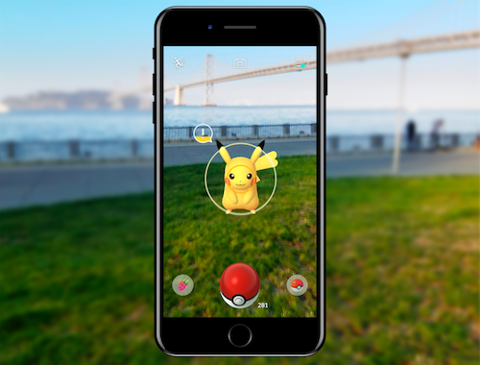
\includegraphics[scale=0.5]{pkmgo}
    \caption[Ejemplo RA]{Ejemplo de Realidad Aumentada en el videojuego Pokémon Go}
\end{figure}

Existen otros términos acuñados que son a grandes rasgos sinónimos de la \textit{RA} como \textit{Mixed Reality}. No debe confundirse con la \textit{Realidad Virtual}, otro ámbito en el que el objetivo es sumergir al usuario en un mundo virtual enajenándolo de sus sentidos con el mundo real, usualmente con unas gafas envolventes diseñadas específicamente para realidad virtual. Todas estas disciplinas están recogidas bajo el término paraguas de la \textit{Extended Reality} (\textit{XR}).

A continuación se van a describir los tipos de escenas que podemos encontrarnos en el contexto de la Realidad Aumentada.

\begin{itemize}
    \item \textbf{Posicionamiento en superficies}: Es quizás el ejemplo más sencillo tanto conceptualmente como técnicamente. El dispositivo intentará analizar sus alrededores a través de la cámara e intentará detectar superficies planas como podría ser una el suelo, una mesa o una pared. Colocará objetos en puntos concretos de estas superficies, y al mover el dispositivo esos objetos deberán visualizarse como si estuvieran colgados o colocados en dichas instancias del mundo real. Existe todavía a día de hoy una limitación importante a la hora de realizar estas escenas; si la superficie es demasiado lisa y uniforme, el dispositivo la reconocerá con gran probabilidad como un color plano, y no tendrá la capacidad de identificarla como una superficie, haciendo que no pueda llegar a colocar nada.
    
    \begin{figure}[h]
        \centering
        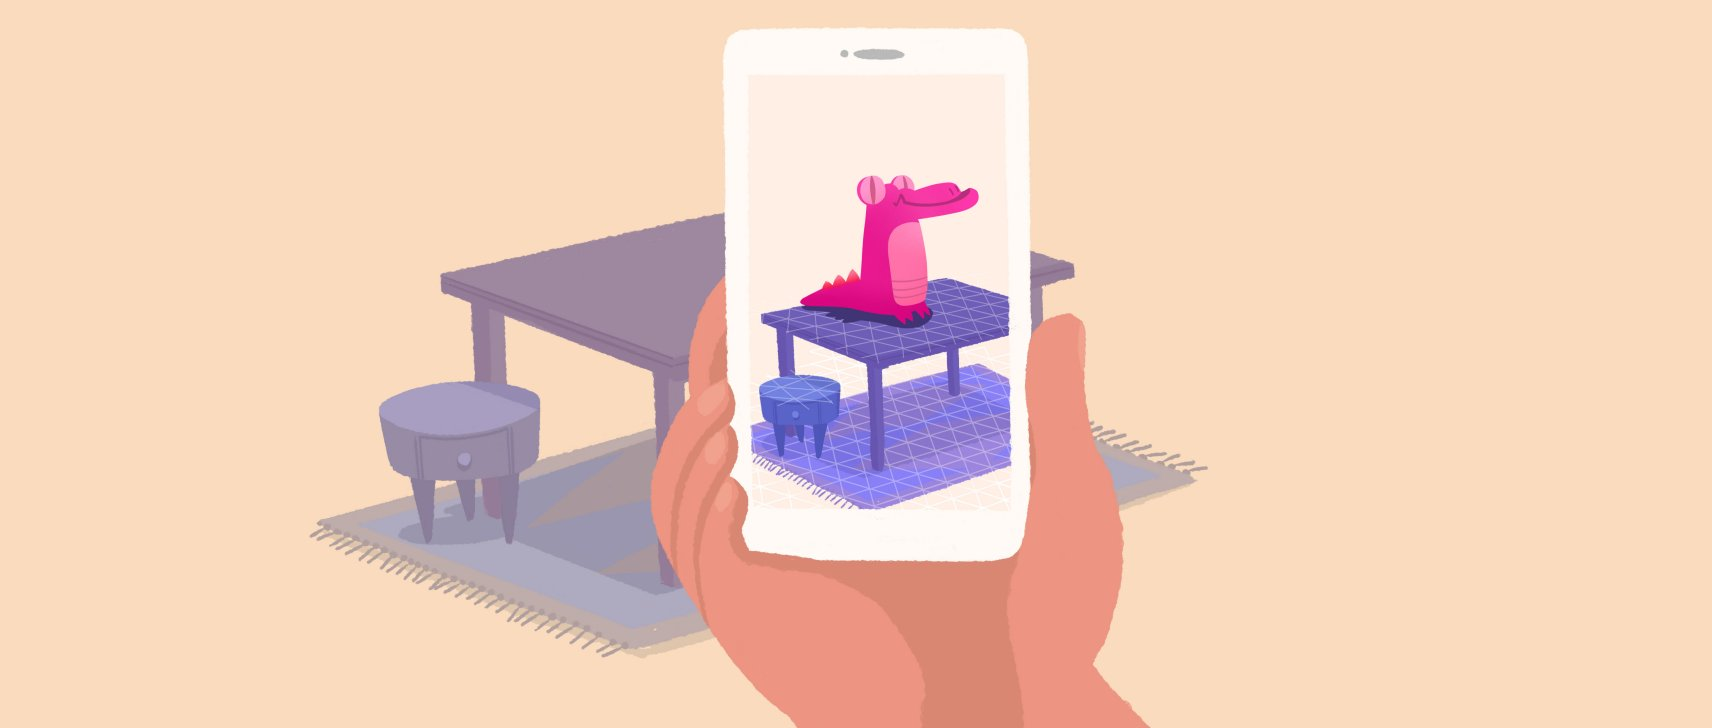
\includegraphics[scale=0.2]{ground}
        \caption[Ejemplo ground]{Ejemplo de posicionamiento en superficies de la documentación de \textit{ARCore}\cite{arcore}}
    \end{figure}

    \item \textbf{Imágenes aumentadas}: En este tipo de escena, cada modelo o conjunto de modelos tiene asociada una imagen bidimensional a la que denominamos \textbf{marcador} o \textbf{activador}. Cuando se inicie, el dispositivo tratará de reconocer esta imagen en el mundo real. Una vez identificada se reproducirán sobre la imagen (tratándola como una superficie) o en una posición relativa a la imagen, los modelos pertinentes que se hayan definido. Es posible definir distintos objetos asociados a distintos marcadores y que solo se reproduzcan los elementos pertinentes.
    
    \begin{figure}[h]
        \centering
        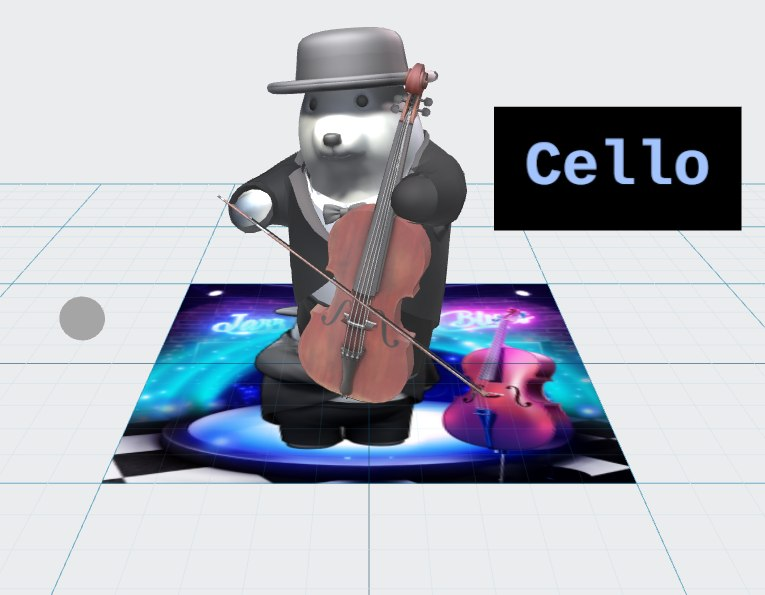
\includegraphics[scale=0.5]{agexample}
        \caption[Ejemplo ground]{Ejemplo de escena de imágenes aumentadas de la web de \textit{Pictarize Studio}\cite{pictarize}}
    \end{figure}

    \item \textbf{Escenas geoespaciales}: Son escenas en las que los objetos no se posicionan en una superficie, si no en unas coordenadas GPS. El usuario solo podrá ver la escena si se encuentra a una latitud, longitud y altura cercanos a aquella que se definieran para la escena. Para ello logicamente es esencial disponer de conexión a internet y que el dispositivo tenga acceso a las coordenadas actuales del usuario durante la ejecución. Las localización GPS de los dispositivos móviles no suele ser del todo precisa, así que usando solo estas es posible que si queremos, por ejemplo, colocar un modelo 3D que represente cómo era la \textit{Alhambra de Granada} cuando se construyó justo en la puerta del edificio, es posible que algunos usuarios la vean algunos metros fuera de lugar, o incluso flotando en el aire. Para poder tener algo más de precisión, algunas APIs geoespaciales como la de \textit{ARCore}\cite{arcore} permiten  extraer información de \textit{Street View}, el visor en primera persona de \textit{Google Maps} para reconocer a través de puntos clave, fachadas de edificios y calles que hayan sido captadas previamente por este servicio, resultando así en una mejor aproximación a la verdadera posición del usuario y por tanto un posicionamiento más preciso de las escenas.

    \begin{figure}[h]
        \centering
        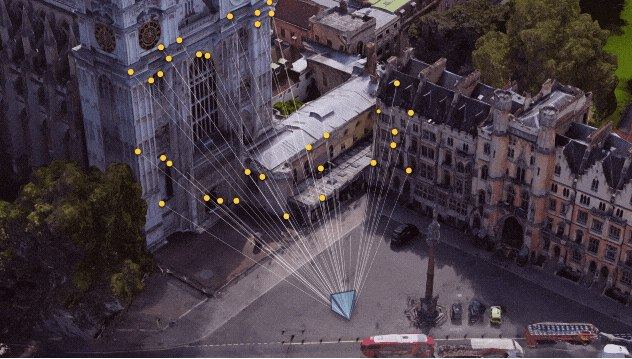
\includegraphics[scale=0.7]{geospatial}
        \caption[Ejemplo ground]{Ejemplo de la aproximación por puntos clave para escenas geoespaciales de la documentación de \textit{ARCore}\cite{arcore}}
    \end{figure}

\end{itemize}


\subsection{Visión por computador}
Javier González Jiménez define en su libro \textit{Visión por computador}\cite{visioncomputador} este campo con la siguiente cita:


    \textit{``La visión por computador, también denominada visión artificial, puede definirse por el proceso de extracción de información del mundo físico a partir de imágenes, utilizando para ello un computador. Desde un punto de vista más ingenieril, un sistema de visión por computador es un sistema autónomo que realiza algunas de las tareas que el sistema de visión humano [...] realiza. La información o tareas que este sistema de visión puede llegar a extraer o realizar puede ir desde la simple detección de objetos sencillos en una imagen hasta \textbf{la interpretación tridimensional de complicadas escenas}.
    ''}

    \textit{``[...] la información visual consiste en energía luminosa procedente del entorno. Para utilizar esa información es preciso transformarla a un formato susceptible de ser procesado [...] esta misma tarea se realiza con una cámara de vídeo (o algún otro dispositivo similar), que convierte la energía luminosa en corriente eléctrica, que puede ser entonces muestreada y digitalizada para su procesamiento en un computador.''}

En nuestro caso nos interesa especialmente la sentencia destacada de la cita. Esta disciplina nos permite extraer una idea de la estructura física de un escenario, permitiéndonos detectar elementos como superficies o esquinas, indispensables si queremos por ejemplo, posicionar un objeto 3D encima de una mesa, y que el objeto parezca que siga apoyado en la mesa si movemos la cámara de lugar, cambiamos el ángulo, o nos alejamos.

Por fortuna la obtención de información a través de imágenes será un proceso completamente transparente para nosotros gracias a las distintas herramientas y tecnologías que ofrecen una API para hacer llamada de estas funciones sin que tengamos que preocuparnos por los detalles técnicos como veremos a continuación.

\subsection{ARCore}
\textit{ARCore}\cite{arcore}  es un \textit{SDK} (\textit{software development kit}) de Realidad Aumentada desarrollado por Google. Ofrece una API con la que se pueden desarrollar experiencias \textit{AR} en Android, iOS, Unity y Web renderizando modelos 3D con \textit{OpenGL}. Para ello ARCore realiza una serie de tareas a bajo nivel relativas a la visión por computador y por las cuales el usuario no tiene que preocuparse, solo hacer las llamadas necesarias a su API. Estas funciones se detallan a continuación.

\begin{itemize}
    \item \textbf{Seguimiento de movimiento}: Se emplea un proceso llamado \textit{localización y asignación simultáneos}, o ANSM, para que el dispositivo obtenga un contexto sobre el mundo físico que lo rodea. Para ello ARCore detecta características visualmente distintas en las imágenes capturadas (también llamadas \textbf{puntos de atributo}) y los usa para calcular el cambio de ubicación del dispositivo. La información visual se combina con la IMU\footnote{Un IMU (Unidad de Medida Inercial) es un dispositivo capaz de estimar y reportar información acerca de la velocidad y orientación del mismo a través de acelerómetros y giroscopios.} del dispositivo para calcular la pose, es decir, la posición y orientación de la cámara respecto al mundo a lo largo del tiempo.

    \item \textbf{Comprensión ambiental}: Búsqueda de clústeres de puntos de atributos que aparentan pertenecer a superficies horizontales o verticales como pareces o mesas, y las pone a disposición del usuario como \textit{planos} que pueden emplearse para posicionar objetos.

    \item \textbf{Comprensión de profundidad}: ARCore detecta y almacena \textit{mapas de profundidad} con información sobre la distancia entre dos puntos cualquiera pertenecientes a una superficie. Esto puede emplearse para simular interacciones físicas realistas entre objetos virtuales y reales o lograr el efecto de que un objeto virtual aparezca tapado o detrás de uno real.

    \item \textbf{Estimación de luz}: Detecta información sobre la luz de su entorno, su intensidad y color. Con esto se pueden lograr efectos como que un objeto virtual a la sombra se represente más oscuro que uno expuesto a una fuente de luz.

    \item \textbf{Estimación de luz}: Detecta información sobre la luz de su entorno, su intensidad y color. Con esto se pueden lograr efectos como que un objeto virtual a la sombra se represente más oscuro que uno expuesto a una fuente de luz.

    \item \textbf{Interacción de usuario}: A través de raycasts\footnote{text raycast}, ARCore puede obtener un \textit{punto de atributo} o modelo posicionado en la escena a partir de un gesto de usuario como tocar la pantalla táctil del dispositivo, lo que permite interacciones como colocar o mover objetos 3D.

    \item \textbf{Puntos orientados}: Los puntos orientados permiten posicionar objetos 3D en superficies que no son superficies planas. ARCore analiza los puntos de atributo vecinos al seleccionado para posicionar el objeto y realizará una estimación de la inclinación, devolviendo un ángulo que servirá para aplicar una pose al objeto para que se vea lo más natural posible.

    \item \textbf{Imágenes aumentadas}: ARCore puede detectar a través de la cámara imágenes 2D definidas previamente y asociar a cada una uno o varios modelos 3D que posicionar sobre estas en el caso de que se enfoquen. Los modelos mantendrán su posición de forma consistente si la cámara se mueve o rota.

\end{itemize}

\subsection{SceneView}

\textbf{Sceneform} es un \textit{SDK} desarrollado por \textit{Google} que permite importar y visualizar modelos 3D en distintos formatos para renderizar escenas 3D para aplicaciones de \textit{ARCore} o realidad virtual sin necesidad de programar código \textit{OpenGL} de bajo nivel. Cuenta con un \textit{grafo de escena} a través del cual podemos definir la estructura de los modelos de la misma a través de un árbol de nodos, y un motor de físicas de \textit{Filamente}\footnote{Filament: Motor de físicas para escenas 3D en tiempo real desarrollado por Google.}.

Lamentablemente, \textit{Sceneform} fue abandonado por \textit{Google}, pero el proyecto ha renacido bajo el nombre de \textbf{Sceneview}\cite{sceneview}, desligándose de \textit{Google}, con código abierto y mantenido por su comunidad.

\subsection{Android y Android Studio}

\textbf{Android} es un sistema operativo desarrollado por Google, de código abierto y basado en el núcleo de \textit{Linux}. En un principio se diseñó con dispositivos táctiles en mente como teléfonos inteligentes y \textit{tablets}. Es el que actualmente tiene la mayor cuota de mercado en dispositivos de este tipo, contando en 2022 con el 72,2\%\footnote{\url{https://root-nation.com/es/noticias-es/es-cuota-mercado-android-ios-estadisticas-publicadas-2022/}}. También se emplea en otro tipo de sistemas como televisiones y relojes inteligentes o incluso automóviles.

\textbf{Android Studio} es un entorno de desarrollo integrado o \textit{IDE}, es decir, una aplicación informática que proporciona servicios y recursos para el desarrollador de software como un editor de código, depurador, compilador e interfaz gráfica. En este caso para el desarrollo de aplicaciones en dispositivos Android. Este tipo de herramientas es de gran interés para encarar un desarrollo, ya que aglutina todas las herramientas que podemos necesitar como programadores en un solo entorno.

\textbf{Kotlin}  es un lenguaje de programación multiplataforma, estáticamente tipado, con inferencia de tipos y de alto nivel. Está diseñado para ser totalmente inter operable con \textit{Java}, pero usando una sintaxis más concisa. Es además, el lenguaje preferido por Google para el desarrollo de aplicaciones Android y el que se recomienda en toda la documentación.

\subsection{Typescript}
\textit{JavaScript} (\textit{JS}) es un lenguaje de programación interpretado y compilado \textit{just-in-time}, aunque es más conocido como un lenguaje de \textit{scripting}, es decir, un lenguaje que nos permite incrustar código dentro de páginas web.

Por otro lado, \textit{TypeScript} (\textit{TS}) es un lenguaje construido por encima de JavaScript que añade sintaxis adicional que lo hace \textbf{fuertemente tipado}. Es decir, siempre que declaremos una variable debemos especificar su tipo. Si más adelante en el código se intenta asignar un valor no correspondiente a ese tipo, el editor podrá detectarlo y avisar, pudiendo así identificar posibles errores antes siquiera de la ejecución del programa, cosa que con \textit{JavaScript} no es posible.

\subsection{Archivo JSON}
Los archivos JSON (o \textit{JavaScript Object Notation}) es un formato de texto sencillo para el intercambio de datos. Toma como referencia la notación de objetos de \textit{JS}, pero a lo largo de los años y debido a su simplicidad, se ha convertido en la opción por defecto para intercambio de información entre servicios web, en contraposición a su principal alternativa, \textit{XML}.

\subsection{Three.js}
\textit{Three.js}\cite{three} es una librerías \textit{JavaScript} usada para crear y renderizar gráficos 3D animados en páginas web para que puedan se reproducidas en un navegador. Para ello hace uso de \textit{WebGL}, otra librería \textit{JavaScript} para la renderización de gráficos pero a más bajo nivel. \textit{Three.js} se abstrae de conceptos técnicos y de bajo nivel para que el desarrollador no tenga que preocuparse de todo eso y agilice su desarrollo. Además es una librería de código abierto mantenida por su comunidad.

\subsection{React.js}
\textit{React}\cite{react} es una librería de \textit{JavaScript} para construir interfaces de usuario web de código abierto y mantenido por su comunidad. Opcionalmente, utiliza ficheros de extensión \textit{.jsx} (\textit{JavaScript Syntax Extension}) para facilitar el desarrollo. Estos son, como su nombre indica, una extensión sintáctica de \textit{JS} que permite insertar código HTML, facilitando así la construcción de interfaces de usuario.

\subsection{Node.js}
\textit{Node}\cite{nodejs} es un entorno de ejecución de \textit{JavaScript} orientado a eventos asíncronos diseñado para crear aplicaciones de red rápidas capaces de manipular grandes cantidades de conexiones concurrentes con una alta escalabilidad para los proyectos.

\subsection{Express}
\textit{Express}\cite{express} es un \textit{``Web application framework minimalista y flexible para Node.js que provee una serie de herramientas para aplicaciones web y móviles.''} como lo definen ellos mismos. Cuenta con una gran variedad de utilidades para llamadas \textit{HTTP} y \textit{middleware}. Cuando hablamos de \textit{middleware} nos referimos a un software a través del cual distintas aplicaciones se comunican entre sí por internet. 

\subsection{Firebase}
\textit{Firebase}\cite{firebase} es un BAAS\footnote{Backend-as-a-service: aplicaciones puestas al servicio de desarrolladores para que estos hagan usos de sus servicios y se centren en desarrollar el frontend de sus apps, siendo innecesario así que creen ni mantengan sus propios backends.} desarrollado por \textit{Google} que pone a disposición de los desarrolladores una serie de herramientas y servicios para facilitar la creación de aplicaciones. Algunas de sus servicios más importantes son:

\begin{itemize}
    \item \textbf{Autenticación}: Soporta autenticación de usuarios usando contraseñas con correo electrónico, número de teléfono, o cuentas de \textit{Google}, \textit{Facebook} y \textit{Twitter} entre otros. Ofrece también encriptación por defecto en la base de datos para contraseñas.
    \item \textbf{Base de datos en tiempo real}: \textit{Firebase} tiene también una base de datos \textbf{no relacional} que se actualiza a tiempo real y se mantiene en línea incluso cuando la aplicación no se está ejecutando.
    \item \textbf{Hosting}: Permite \textit{hostear} aplicaciones web de forma fácil y rápida, pudiendo almacenar contenido en una memoria caché y accesible desde cualquier parte del mundo.
\end{itemize}

\subsection{Archivo GLB}
\textbf{GLB} (\textit{.glb}) es un formato de archivo binario estandarizado para representar datos de objetos 3D como modelos, escenas, iluminación, materiales, jerarquías y animaciones. Sus siglas significan \textit{GL Transsmission Format Binary File}. Fue introducido en 2015 como una versión binaria de los ficheros \textbf{GLTF} (\textit{.gltf}), un formato basado en la notación \textit{JSON} muy usado en aplicaciones web y móvil debido a su ligero peso.